\documentclass[12pt]{article}
\usepackage[spanish]{babel}
\usepackage[utf8]{inputenc}     % Para que acepte acentos y ñ directamente
\usepackage[T1]{fontenc}        % Mejor manejo de caracteres acentuados
\usepackage{geometry}
\geometry{a4paper, margin=1in}
\usepackage{graphicx}
\usepackage{xcolor}
\usepackage{titlesec}
\usepackage{parskip}
\usepackage{multicol}
\usepackage{cite}
\usepackage{hyperref}           % Para hipervínculos en PDF
\hypersetup{
  colorlinks=true,
  linkcolor=blue,
  citecolor=blue,
  urlcolor=blue
}
\definecolor{highlight}{RGB}{255, 255, 0}

\titleformat{\section}{\normalfont\Large\bfseries}{\thesection}{1em}{}
\titleformat{\subsection}{\normalfont\large\bfseries}{\thesubsection}{1em}{}

\begin{document}

% Logos
\begin{minipage}{0.45\textwidth}
    
\includegraphics[width=0.4\textwidth]{inFiles/Figures/epnLogo.jpg}
\end{minipage}
\hfill
\begin{minipage}{0.45\textwidth}
    \raggedleft
    
\includegraphics[width=0.4\textwidth]{inFiles/Figures/FIS_logo.jpg}
\end{minipage}

\vspace{0.5cm}

% Títulos principales
\begin{center}
    \textbf{ESCUELA POLITÉCNICA NACIONAL}\\[0.2cm]
    \textbf{FACULTAD DE INGENIERÍA DE SISTEMAS}\\[0.2cm]
    \textbf{INGENIERÍA {\textbf{EN COMPUTACION}}}
\end{center}

\vspace{0.5cm}
\hrule
\vspace{0.5cm}

% Datos principales
\noindent\textbf{PERÍODO ACADÉMICO:} 2025-A\\[0.2cm]
\noindent\textbf{ASIGNATURA:} ICCD412 Métodos Numéricos \hfill \textbf{GRUPO:} GR2\\[0.2cm]
\noindent\textbf{TIPO DE INSTRUMENTO:} {Practica 1}\\[0.2cm]
\noindent\textbf{FECHA DE ENTREGA LÍMITE:}{04/05/2025}\\[0.2cm]
\noindent\textbf{ALUMNO:} {Lema Luis}

\vspace{0.5cm}
\hrule
\vspace{1cm}


% Secciones
\section*{TEMA}
{Tipos de errores}

\vspace{0.5cm}

\section*{OBJETIVOS}
\begin{itemize}
    \item {Analizar con profundidad los errores absoluto y relativo como herramientas clave para evaluar la precisión de los resultados numéricos,
     reconociendo su importancia en la toma de decisiones técnicas fundamentadas.}

     \item {Reflexionar sobre el impacto que tienen los errores de redondeo y truncamiento en los cálculos realizados por medios computacionales, 
     entendiendo cómo estas pequeñas variaciones pueden transformar el resultado final.}
\end{itemize}

\vspace{0.5cm}

\section*{MARCO TEÓRICO}
{Cuando se trabaja con aproximaciones numéricas, es común que los resultados no sean exactos.
 Para medir cuán lejos está una aproximación del valor real, usamos dos conceptos: error absoluto,
  que es la diferencia directa entre el valor real y el aproximado, 
  y error relativo, que compara esa diferencia con el valor real para saber qué tan grande es el error en proporción. 
  Estas dos medidas nos ayudan a evaluar la precisión de nuestros cálculos.} \cite{fisicalabErrores}

  {Para calcular algunos valores como e, se usan herramientas como la serie de Taylor, que permite representar funciones 
  complejas como sumas de términos más simples. Aunque no podemos sumar infinitos términos, 
  usar unos cuantos ya nos da una buena estimación.} \cite{economipediaTaylor}

  {También es importante entender los errores de redondeo, que ocurren al limitar los decimales en los cálculos,
   y los errores de truncamiento, que aparecen cuando cortamos una operación antes de terminarla (como una suma infinita).
    Ambos pueden afectar los resultados si no se controlan bien. } \cite{uaRedondeo}
 

\vspace{0.5cm}

\section*{DESARROLLO}
\begin{minipage}{0.95\textwidth}
    \raggedleft
    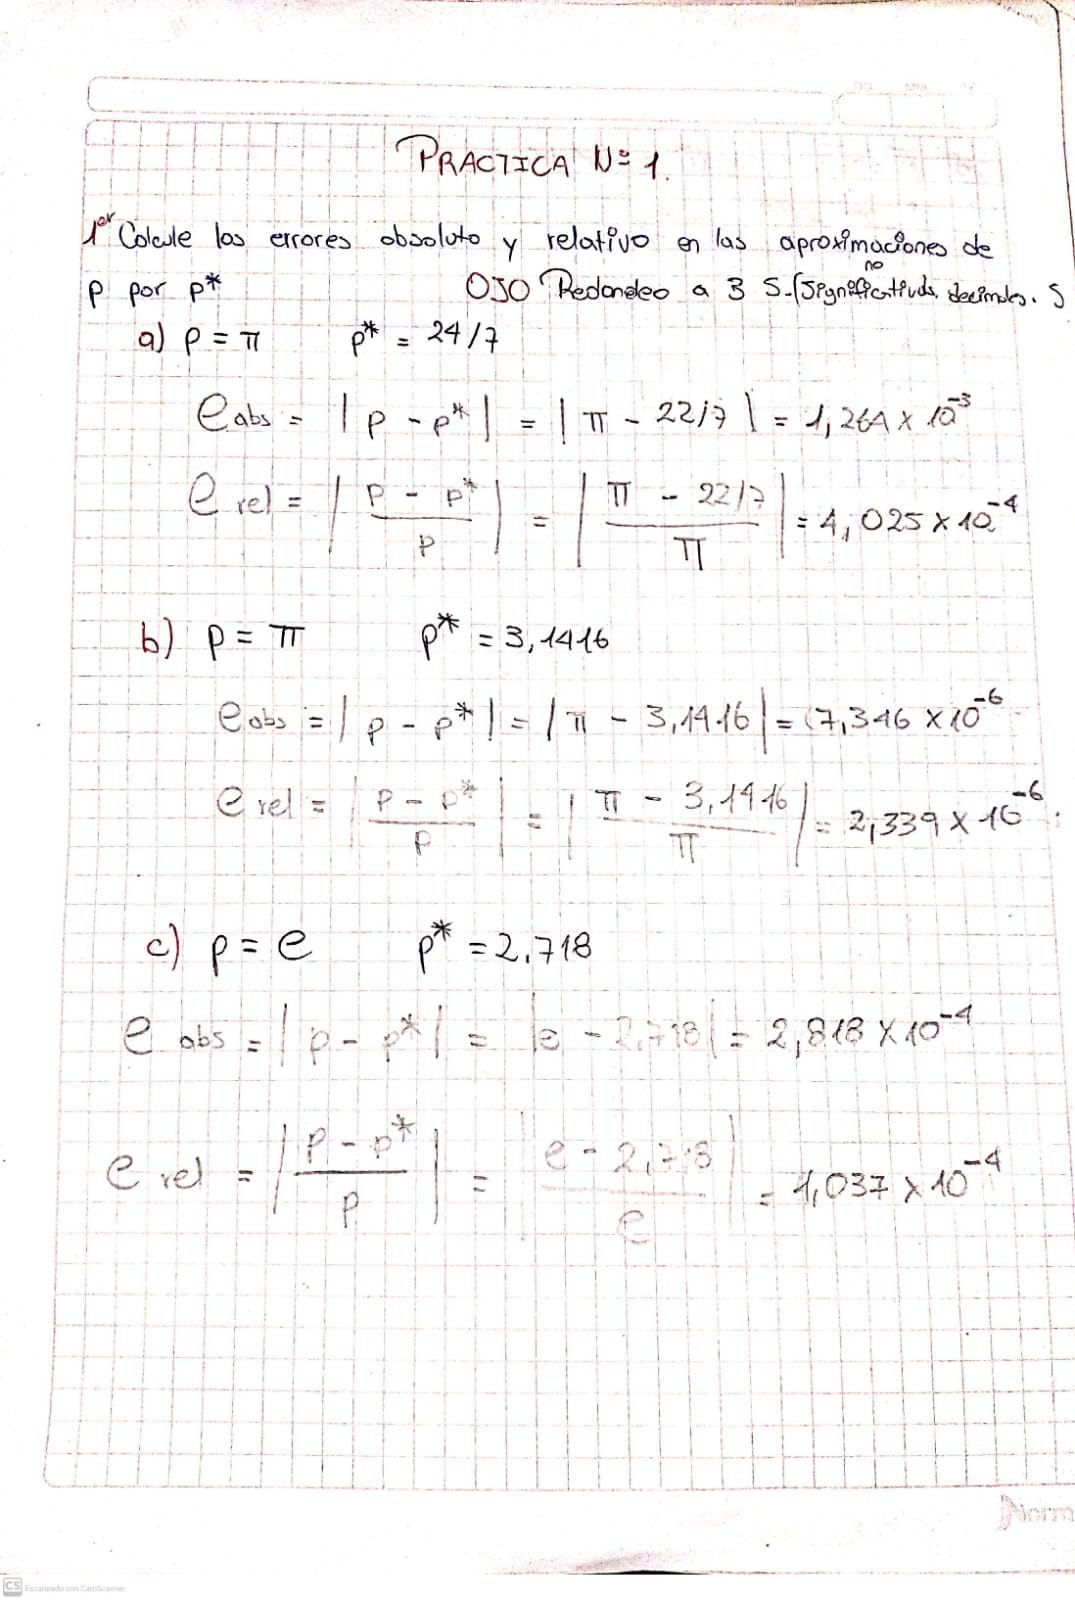
\includegraphics[width=0.95\textwidth]{inFiles/Figures/ej1.jpeg}
\end{minipage}

\vspace{0.5cm}

\begin{minipage}{0.95\textwidth}
    \raggedleft
    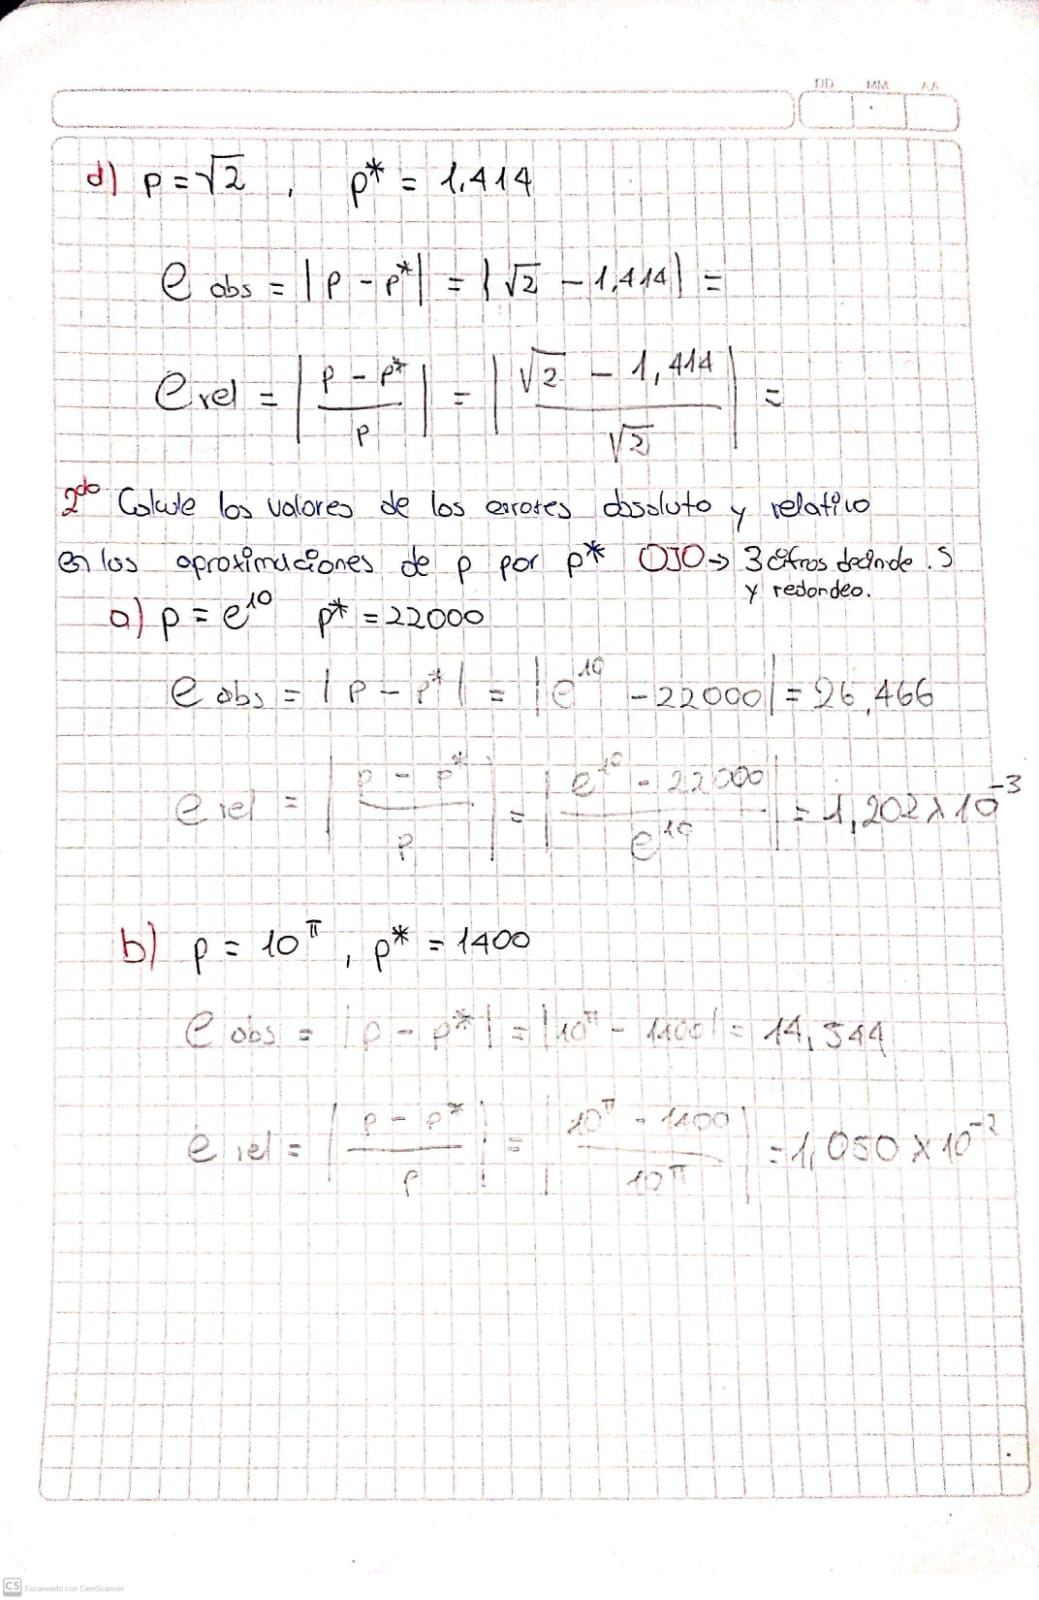
\includegraphics[width=0.95\textwidth]{inFiles/Figures/ej2.jpeg}
\end{minipage}

\vspace{0.5cm}

\begin{minipage}{0.95\textwidth}
    \raggedleft
    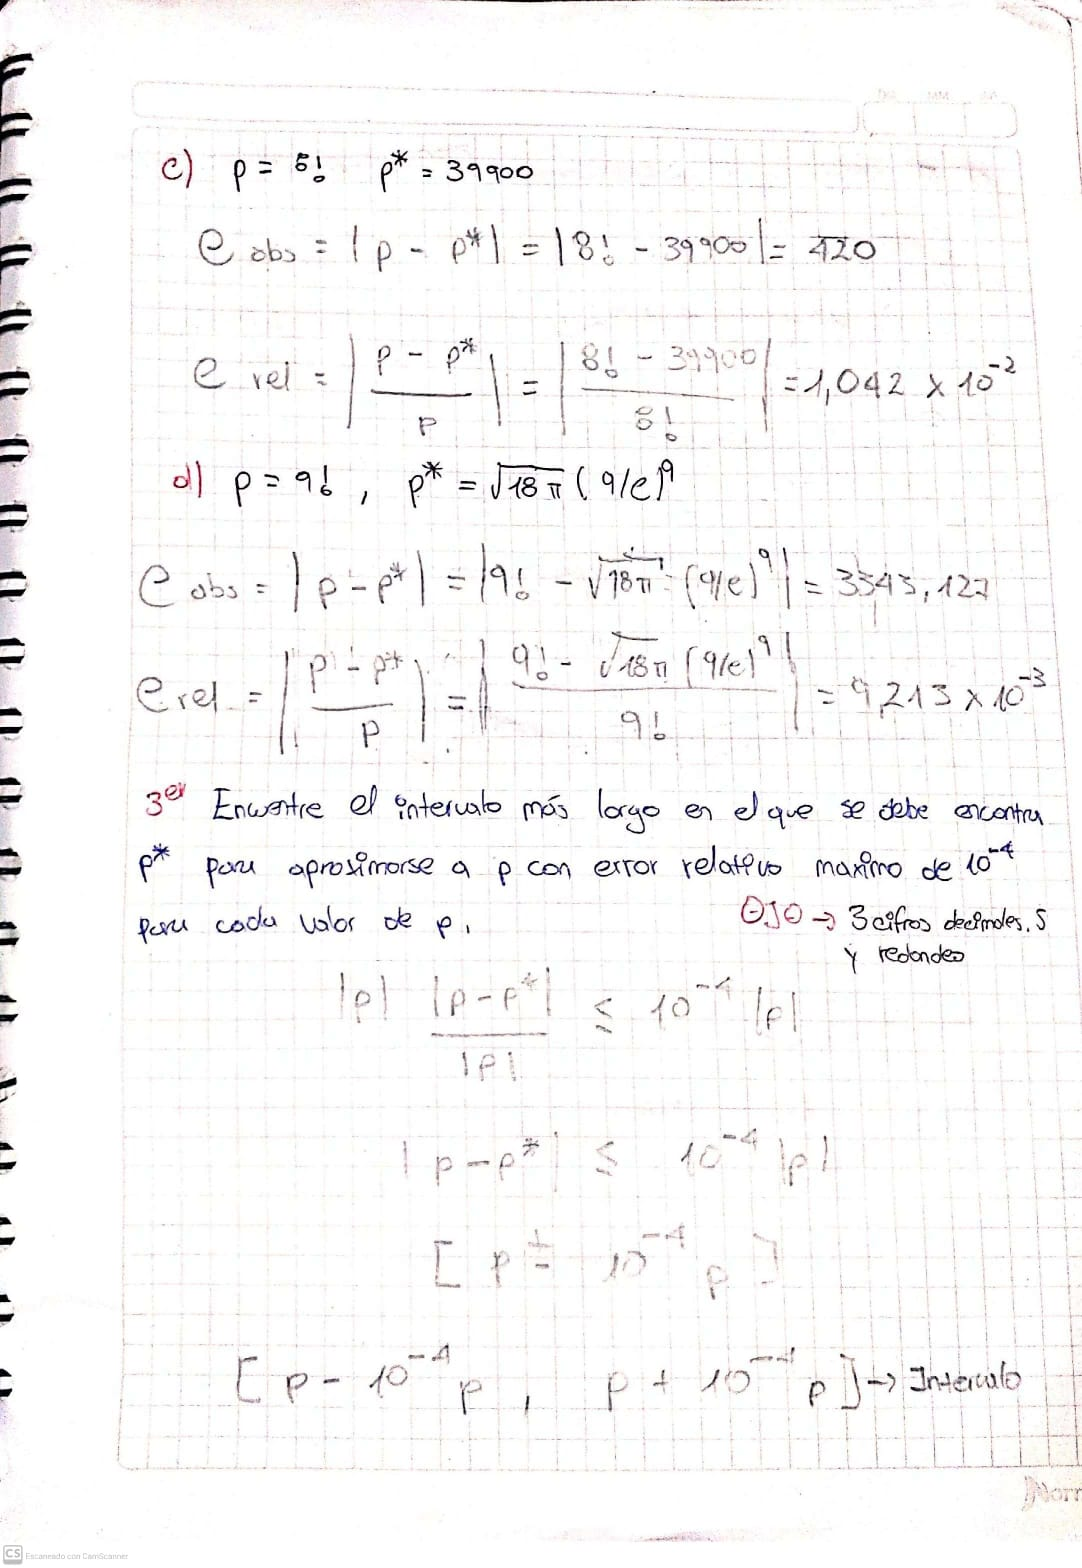
\includegraphics[width=0.95\textwidth]{inFiles/Figures/ej3.jpeg}
\end{minipage}

\vspace{0.5cm}

\begin{minipage}{0.95\textwidth}
    \raggedleft
    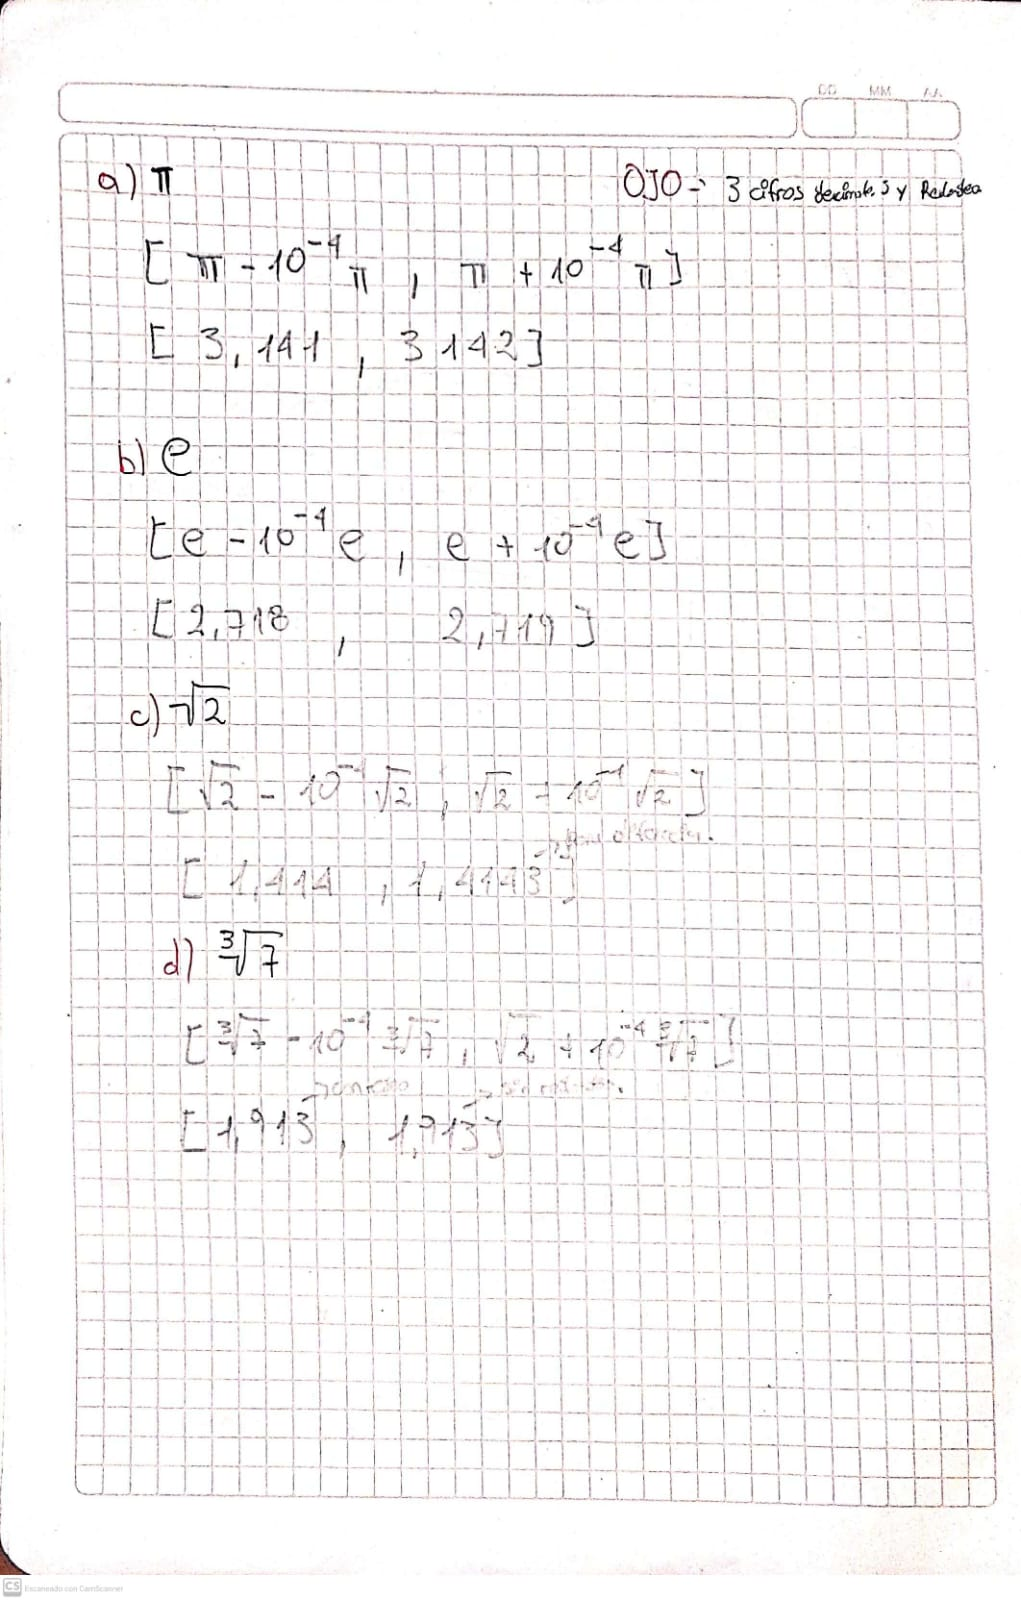
\includegraphics[width=0.95\textwidth]{inFiles/Figures/ej4.jpeg}
\end{minipage}

\vspace{0.5cm}

\begin{minipage}{0.95\textwidth}
    \raggedleft
    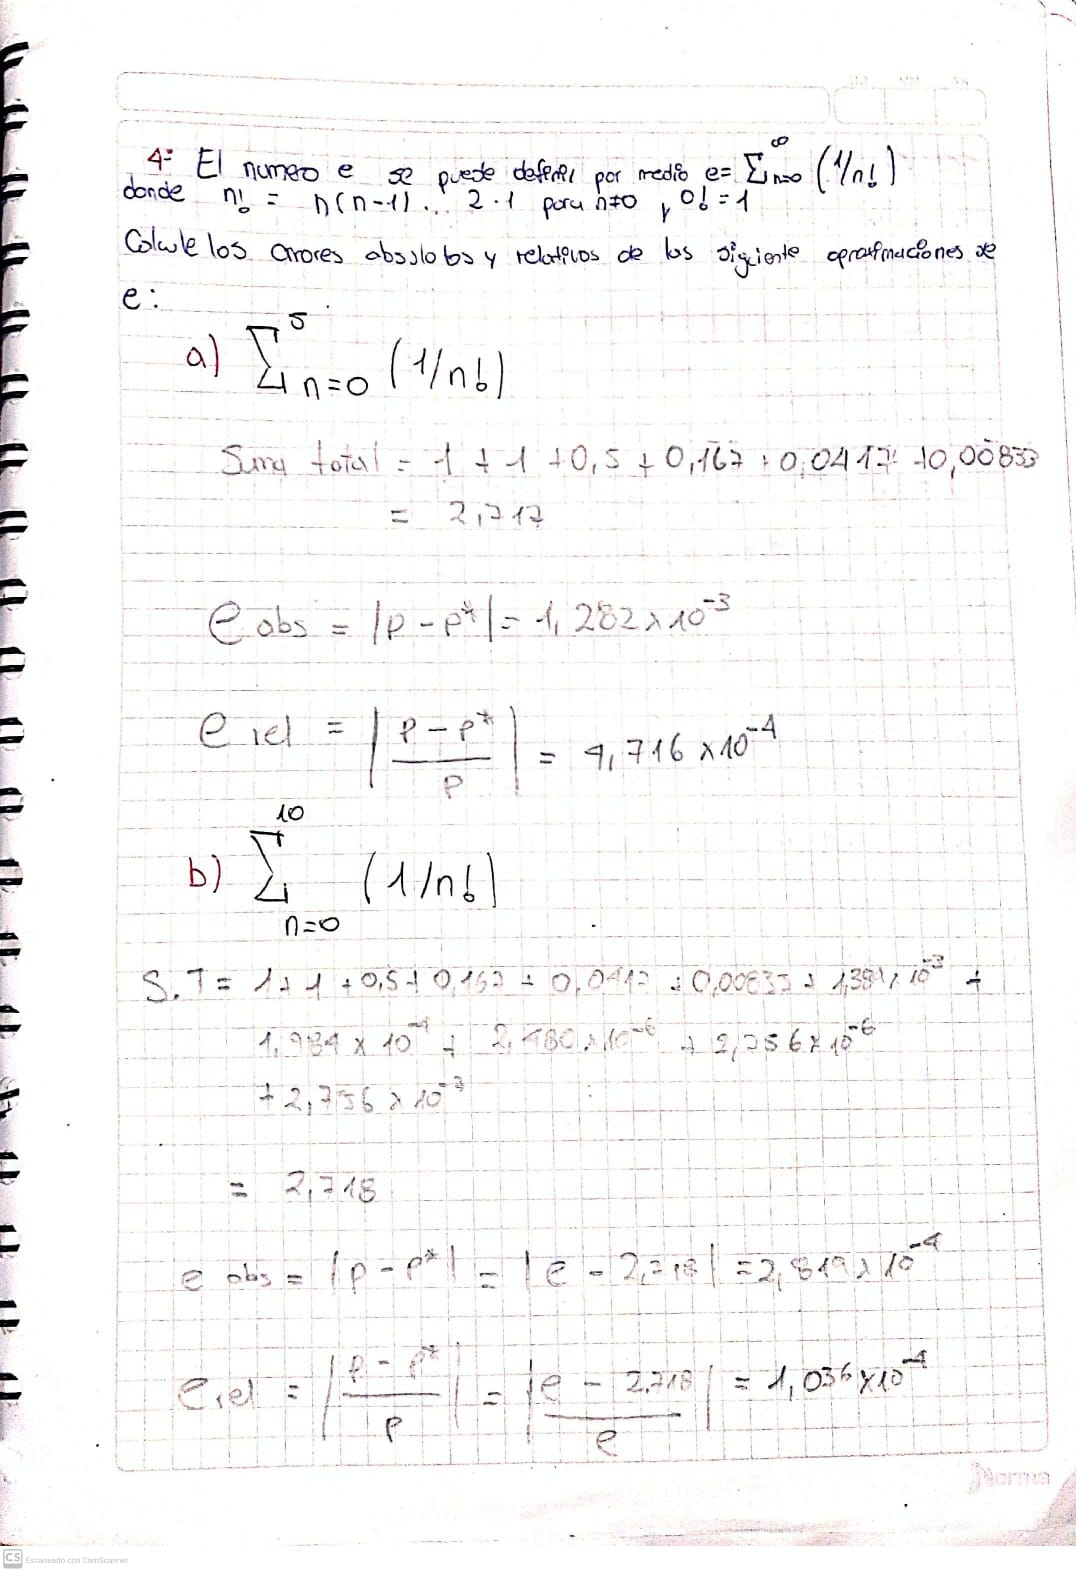
\includegraphics[width=0.95\textwidth]{inFiles/Figures/ej5.jpeg}
\end{minipage}

\vspace{0.5cm}

\begin{minipage}{0.95\textwidth}
    \raggedleft
    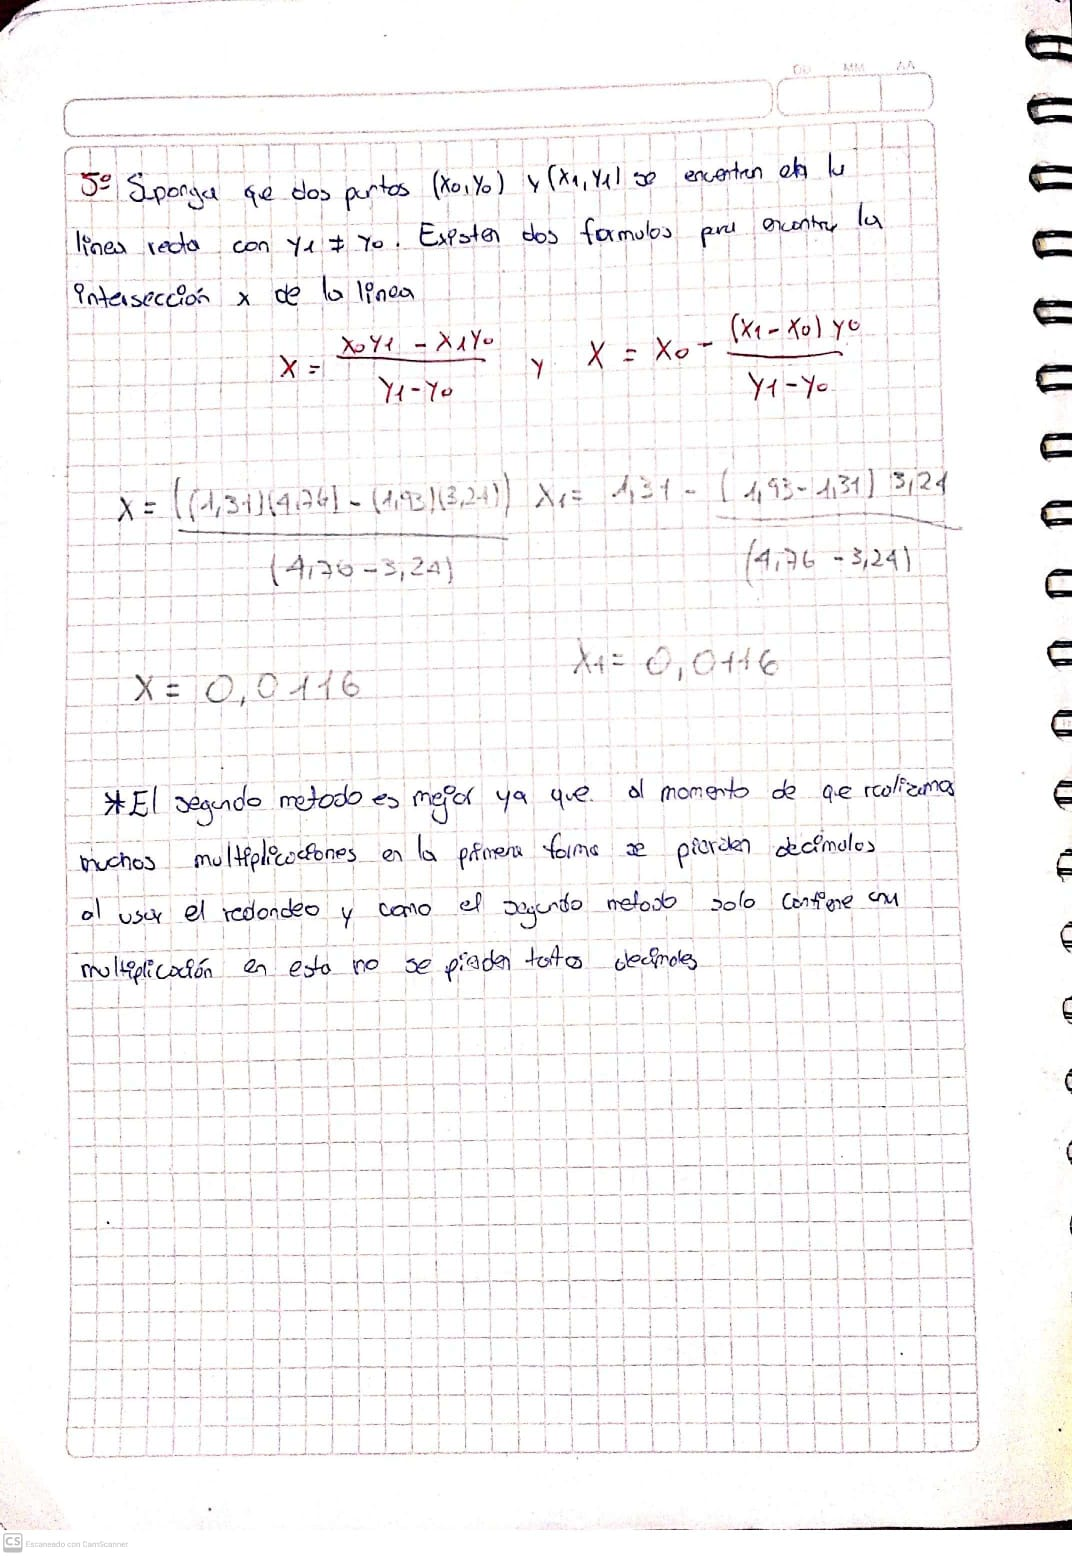
\includegraphics[width=0.95\textwidth]{inFiles/Figures/ej6.jpeg}
\end{minipage}

\vspace{3cm}


\section*{CONCLUSIONES}
\begin{itemize}
    \item {Al hacer esta práctica me di cuenta de que trabajar con números aproximados es más común de lo que parece, pero también hay que tener cuidado con los errores que se generan. 
    Aprender a calcular el error absoluto y el relativo me ayudó a entender mejor si una aproximación es buena o no.}

     \item {Otra cosa que me pareció interesante fue cómo los errores de redondeo y truncamiento afectan los resultados, sobre todo cuando uno trabaja con pocos decimales. 
     Es algo que antes no tomaba tanto en cuenta, pero ahora entiendo que puede cambiar bastante el resultado final.}
\end{itemize}


\vspace{0.5cm}

\section*{RECOMENDACIONES}
\begin{itemize}

     \item {Revisar siempre qué tan buena es una aproximación usando los errores absoluto y relativo.}
     \item {No usar un valor aproximado solo porque “se ve bien”; es mejor comprobar si sirve para lo que se necesita}
     \item {Tener cuidado con los decimales y el redondeo, especialmente en cálculos con muchos pasos.}
     \item {Usar varias formas de hacer el mismo cálculo ayuda a comparar y ver cuál da resultados más confiables.}
     \item {Practicar estos ejercicios más seguido ayuda a entender mejor cómo y cuándo aplicar aproximaciones.}
\end{itemize}


\vspace{0.5cm}


\renewcommand{\refname}{\MakeUppercase{REFERENCIAS}}
\bibliographystyle{IEEEtran}
\bibliography{inFiles/References/references.bib}
\end{document}
